% !TEX program = xelatex
\documentclass{VUMIFPSkursinis}
\usepackage{algorithmicx}
\usepackage{algorithm}
\usepackage{algpseudocode}
\usepackage{amsfonts}
\usepackage{amsmath}
\usepackage{bm}
\usepackage{caption}
\usepackage{color}
\usepackage{float}
\usepackage{graphicx}
\usepackage{listings}
\usepackage{subfig}
\usepackage{array}
\usepackage{wrapfig}

\usepackage{hyperref}
\usepackage{multirow}
\usepackage{longtable}

% Titulinio aprašas
\university{Vilniaus universitetas}
\faculty{Matematikos ir informatikos fakultetas}
\department{}
\papertype{Reikalavimų inžinerijos laboratorinis darbas}
\title{Reikalavimų specifikacija}
\titleineng{Requirement specification}
\status{1 kurso magistratūros studentai}
\author{Šarūnas Kazinieras Buteikis}
\secondauthor{Matas Savickis}
\thirdauthor{Rokas Ulickas}
\fourthauthor{Vytautas Krivickas}
\supervisor{dr. Audronė Lupeikienė}
\date{Vilnius – \the\year}

% Nustatymai
% \setmainfont{Palemonas} % Pakeisti teksto šriftą į Palemonas (turi būti įdiegtas sistemoje)
\bibliography{bibliografija}

\begin{document}

\maketitle

\sectionnonumnocontent{Santrauka}

Šiame dokumente pateikiama „Epidemiologinės šalies sitaucijos sekimo sistemos“
reikalavimų specifikacija. Komandą sudarė:
\begin{itemize}
	\item Šarūnas Kazinieras Buteikis (el. paštas \href{mailto:sarunas.buteikis@mif.stud.vu.lt}{sarunas.buteikis@mif.stud.vu.lt}) -- dokumento maketavimas, taisymai  {\color{red}<...>}
	\item Vytautas Krivickas (el. paštas \href{mailto:vytautas.krivickas@mif.stud.vu.lt}{vytautas.krivickas@mif.stud.vu.lt}) -- dokumento maketavimas, įžanga, {\color{red}<...>}
	\item Matas Savickis (el. paštas \href{mailto:matas.savickis@mif.stud.vu.lt}{matas.savickis@mif.stud.vu.lt}) -- dokumento maketavimas, {\color{red}<...>}
	\item Rokas Ulicas (el. paštas \href{mailto:rokas.ulickas@mif.stud.vu.lt}{rokas.ulickas@mif.stud.vu.lt}) -- {\color{red}<...>}
\end{itemize}

\newpage

\tableofcontents

\section{Įžanga}
Šiame dokumente aprašoma “Epidemiologinės šalies sitaucijos sekimo sistema”, toliau - “sistema”.
Ši sistema skirta sekti epidemiologinei padėčiai šalyje: įvertinti viruso plitimo šalyje tendencijas,
efektyviai identifikuoti naujus viruso židinius, leisti specialistams atsekti susirgusiųjų
kontaktus registruojant užsikrėtusiųjų maršrutus ir potencialiuose rizikos židiniuose
besilankančius žmones, greitai informuoti kontaktavusiuosius su užsikrėtusiu žmogumi
apie privalomą saviizoliaciją, rinkti duomenis apie asmenis karantine.

\subsection{Application domain}
Ši sistema skirta naudoti sveikatos apsaugos sistemoje: sistema turėtų palengvinti
epidemiologų darbą ir leisti sekti viruso plitimą populiacijoje, imtis efektyvesnės
profilaktikos ir tirti naudojamų priemonių efektyvumą.

\subsection{Problem domain}
Sistema siekiama išspręsti šias problemas:
\begin{itemize}
	\item Atskirų sveikatos įstaigų renkami susirgimų duomenys nėra apdorojami centralizuotai
	      arba tai daroma ne sistemingai, todėl epidemiologams sunku identifikuoti tikrąsias viruso
	      plitimo šalyje tendencijas, greitai identifikuoti potencialius židinius.
	\item Dėl žmogiškųjų resursų trūkumo dažnai tampa neįmanoma įspėti visų kontaktavusiųjų
	      su užsikrėtusiuoju asmenų - automatizavus šį procesą būtų galima įgyvendinti efektyvesnę
	      profilaktiką, užkardyti nevaldomą epidemijos plitimą.
	\item Šiuo metu nėra centralizuotos sistemos, leidžiančios registruoti potencialiuose
	      rizikos židiniuose (įvairuose renginiuose, masinio susibūrimo vietose) besilankančius
	      asmenis, dabar egzistuojančios pavienės iniciatyvos neleidžia automatiškai atsekti reikšmingo kiekio susirgusiojo kontaktų - tenka pasikliauti pastarojo pateikta informacija.
	\item Nacionalinio sveikatos centro darbuotojai neturi galimybės automatiškai įspėti
	      atvykusiųjų iš pavojingų šalių asmenų apie privalomą saviizoliaciją: atlikus reikiamas
	      integracijas su {\color{red}muitinės (?)} sistemomis ši sistema leistų automatizuoti ir šį procesą.
	\item Šiuo metu nėra galimybės automatizuoti saviizoliacijos reikalavimų laikymosi sekimo,
	      tad naujoji sistema leistų bent iš dalies automatizuoti šį procesą: reikalauti asmenis
	      saviizoliacijoje pateikti savo dabartinę vietą naudojantis išmaniajame telefone esančia
	      GPS sistema ar atsiųsti saviizoliaciją patvirtinančią nuotrauką.
\end{itemize}

\subsection{Naudotojai}
Šios sistemos naudotojų bazę sudaro trijų kategorijų naudotojai:
\begin{itemize}
	\item Epidemiologai - tai savo srities ekspertai, turintys aukštąjį išsilavinimą.
	      Naudotis sistema jiems pakaks mokykloje dėstomo informatikos kurso.
	\item LR esantys asmenys, dalyvaujantys riziką turinčiuose renginiuose, esantys saviizoliacijoje,
	      atvykę iš pavojingų šalių ar turėję sąlytį su sergančiaisiais - jiems taip pat pakaks
	      mokykloje dėstomo informatikos kurso.
	\item Duomenų analitikai - tam, jog galėtų efektyviai panaudoti sistemoje
	      esančius duomenis jiems reikalingas bakalauro ar aukštesnis iššsilavinimas
	      duomenų mokslo ar informatikos srityse.
\end{itemize}

\newpage

\section{Reikalavimų artefaktai}

\begin{table}[h!]
	\begin{tabular}{|p{4cm}|p{4cm}|p{4cm}|p{4cm}|}
		\hline
		                          & Kodėl? (motyvacija) & \multicolumn{1}{c|}{Kaip? (veiklos)} & Ką? (apdorojami objektai) \\ \hline
		\begin{tabular}[c]{@{}l@{}}Veikslo reikalavimai \\ (verslo inžinieriaus \\ požiūris)\end{tabular} &                     &
		1. Tvarkyti visą informaciją susijusią su žmonėmis
		sergančiais koronos virusu ir informuoti pacientus
		apie jų seikatos būklę bei galimas virusinio susirgimo rizikas.
		2. Galimybė tvarkyti pacientų užsikrėtimų įrašus.
		3. Galimybė pacientui paskirti viruso tyrimą.
		4. Galimybė pacientui paskirti viruso antikūnių tyrimą.
		5. Galimybė pacientui pranešti apie viruso tyrimo rezultatus.																																6. Galimybė registruoti paciento buvimo vietas.
		7. Galimybė pacientui praneši apie viruso židinius.
		8. Galimybė pacientui paskirti vakciną.
		9. Galimybė pacientui paskirti gydymą.
		10. Galimybė registruoti paciento gydymo eigą.




		                          &                                                                                        \\ \hline
	\end{tabular}
\end{table}

\begin{table}[h!]
	\begin{tabular}{|p{4cm}|p{4cm}|p{4cm}|p{4cm}|}\hline
		                          & Kodėl? (motyvacija) & \multicolumn{1}{c|}{Kaip? (veiklos)} & Ką? (apdorojami objektai) \\ \hline
		\begin{tabular}[c]{@{}l@{}}Vartotojo reikalavimai \\ (dalykinės srities \\ specialisto požiūris)\end{tabular} &                     &                                      &                           \\ \hline
	\end{tabular}
\end{table}

\begin{table}[h!]
	\begin{tabular}{|p{4cm}|p{4cm}|p{4cm}|p{4cm}|}\hline
		                          & Kodėl? (motyvacija) & \multicolumn{1}{c|}{Kaip? (veiklos)} & Ką? (apdorojami objektai) \\ \hline
		\begin{tabular}[c]{@{}l@{}}IS reikalavimai \\ (IS inžinieriaus \\ požiūris)\end{tabular} &                     &                                      &                           \\ \hline
	\end{tabular}
\end{table}

\begin{table}[h!]
	\begin{tabular}{|p{4cm}|p{4cm}|p{4cm}|p{4cm}|}\hline
		                          & Kodėl? (motyvacija) & \multicolumn{1}{c|}{Kaip? (veiklos)} & Ką? (apdorojami objektai) \\ \hline
		\begin{tabular}[c]{@{}l@{}}PS reikalavimai \\ (sisteminio analitiko \\ požiūris)\end{tabular} &                     &                                      &                           \\ \hline
	\end{tabular}
\end{table}

\begin{table}[h!]
	\begin{tabular}{|p{4cm}|p{4cm}|p{4cm}|p{4cm}|}\hline
		                          & Kodėl? (motyvacija) & \multicolumn{1}{c|}{Kaip? (veiklos)} & Ką? (apdorojami objektai) \\ \hline
		\begin{tabular}[c]{@{}l@{}}Projektiniai PS \\ reikalavimai \\ (PS inžinieriaus \\ požiūris)\end{tabular} &                     &                                      &                           \\ \hline
	\end{tabular}
\end{table}

\begin{table}[h!]
	\begin{tabular}{|p{4cm}|p{4cm}|p{4cm}|p{4cm}|}\hline
		                          & Kodėl? (motyvacija) & \multicolumn{1}{c|}{Kaip? (veiklos)} & Ką? (apdorojami objektai) \\ \hline
		\begin{tabular}[c]{@{}l@{}}Realizaciniai PS \\ reikalavimai \\ (programuotojo požiūris)\end{tabular} &                     &                                      &                           \\ \hline
	\end{tabular}
\end{table}

\begin{table}[h!]
	\begin{tabular}{|l|l|l|l|}\hline
		                           & Kas? (funkciniai vienetai) & \multicolumn{1}{c|}{Kur? (vieta)} & Kada? (laikas) \\ \hline
		\begin{tabular}[c]{@{}l@{}}Veikslo reikalavimai \\ (verslo inžinieriaus \\ požiūris)\end{tabular} &                            &                                   &                \\ \hline
	\end{tabular}
\end{table}

\begin{table}[h!]
	\begin{tabular}{|l|l|l|l|}\hline
		                           & Kas? (funkciniai vienetai) & \multicolumn{1}{c|}{Kur? (vieta)} & Kada? (laikas) \\ \hline
		\begin{tabular}[c]{@{}l@{}}Vartotojo reikalavimai \\ (dalykinės srities \\ specialisto požiūris)\end{tabular} &                            &                                   &                \\ \hline
	\end{tabular}
\end{table}

\begin{table}[h!]
	\begin{tabular}{|l|l|l|l|}\hline
		                           & Kas? (funkciniai vienetai) & \multicolumn{1}{c|}{Kur? (vieta)} & Kada? (laikas) \\ \hline
		\begin{tabular}[c]{@{}l@{}}IS reikalavimai \\ (IS inžinieriaus \\ požiūris)\end{tabular} &                            &                                   &                \\ \hline
	\end{tabular}
\end{table}

\begin{table}[h!]
	\begin{tabular}{|l|l|l|l|}\hline
		                           & Kas? (funkciniai vienetai) & \multicolumn{1}{c|}{Kur? (vieta)} & Kada? (laikas) \\ \hline
		\begin{tabular}[c]{@{}l@{}}PS reikalavimai \\ (sisteminio analitiko \\ požiūris)\end{tabular} &                            &                                   &                \\ \hline
	\end{tabular}
\end{table}

\begin{table}[h!]
	\begin{tabular}{|l|l|l|l|}\hline
		                           & Kas? (funkciniai vienetai) & \multicolumn{1}{c|}{Kur? (vieta)} & Kada? (laikas) \\ \hline
		\begin{tabular}[c]{@{}l@{}}Projektiniai PS \\ reikalavimai \\ (PS inžinieriaus \\ požiūris)\end{tabular} &                            &                                   &                \\ \hline
	\end{tabular}
\end{table}

\begin{table}[h!]
	\begin{tabular}{|l|l|l|l|}\hline
		                           & Kas? (funkciniai vienetai) & \multicolumn{1}{c|}{Kur? (vieta)} & Kada? (laikas) \\ \hline
		\begin{tabular}[c]{@{}l@{}}Realizaciniai PS \\ reikalavimai \\ (programuotojo požiūris)\end{tabular} &                            &                                   &                \\ \hline
	\end{tabular}
\end{table}


\section{Verslo reikalavimai}

\subsection{Kodėl?}

\begin{figure}[H]
    \centering
    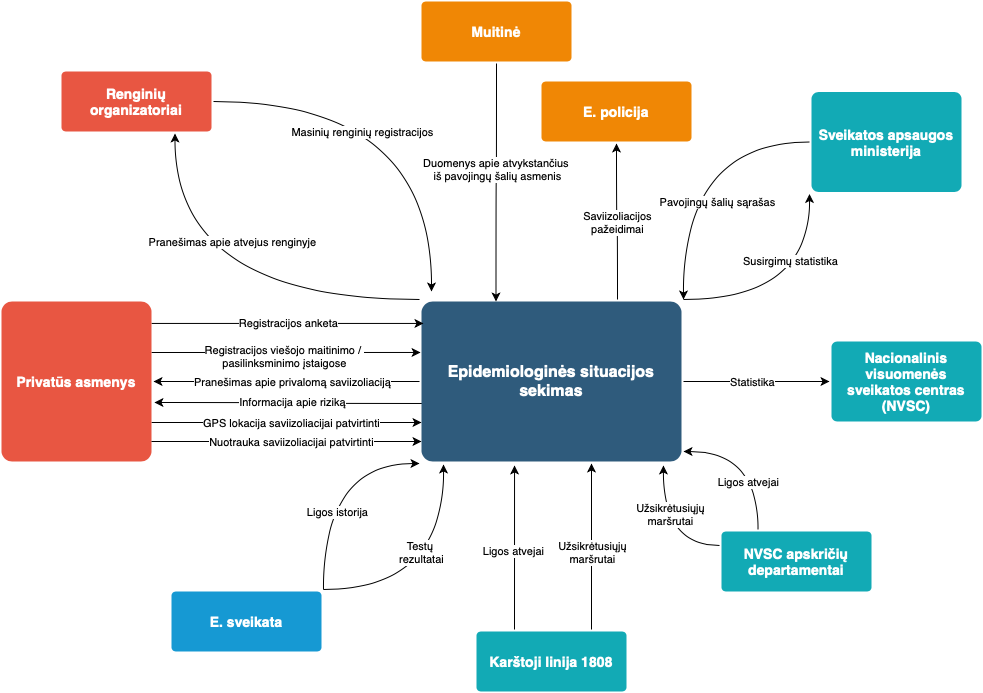
\includegraphics[scale=0.4]{img/context_diagram.png}
    \caption{Konteksto diagrama}
    \label{img:context_diagram}
\end{figure}

\subsubsection{Išorinė verslo analizė}



\subsubsection{Įvestys}

\begin{table}[]
	\centering
	\resizebox{\textwidth}{!}{%
		\begin{tabular}{|l|l|l|l|l|}
			\hline
			\textbf{Nr.}        & \textbf{Įvestis}                                            & \multicolumn{1}{c|}{\textbf{Įvertinimo parametrai}} & \multicolumn{1}{c|}{\textbf{Kiekybiniai matai}} & \multicolumn{1}{c|}{\textbf{Kokybiniai matai}} \\ \hline
			\multirow{2}{*}{I1} & \multirow{2}{*}{Registracijos didesnės rizikos renginiuose} & Kiekis                                              &                                                 &                                                \\ \cline{3-5}
			                    &                                                             & Korektiškumas                                       &                                                 &                                                \\ \hline
			I2                  & Registracijos viešojo maitinbimo įstaigose                  &                                                     &                                                 &                                                \\ \hline
			I3                  & Informacija apie keliones iš rizikos šalių                  &                                                     &                                                 &                                                \\ \hline
			I4                  & Pavojingų šalių sąrašas                                     &                                                     &                                                 &                                                \\ \hline
			I5                  & Asmenų ligos istorijos                                      &                                                     &                                                 &                                                \\ \hline
			I6                  & Testų rezultatai                                            &                                                     &                                                 &                                                \\ \hline
			I7                  & Saviizoliaciją patvirtinantys vietos nustatymo duomenys     &                                                     &                                                 &                                                \\ \hline
			I8                  & Saviizoliaciją patvirtinanti nuotrauką                      &                                                     &                                                 &                                                \\ \hline
			I9                  & Atvykusių iš pavojingų šalių žmonių sąrašas                 &                                                     &                                                 &                                                \\ \hline
			I10                 & Masinių renginių registracijos                              &                                                     &                                                 &                                                \\ \hline
			I11                 & Užsikrėtusiųjų maršrutai                                    &                                                     &                                                 &                                                \\ \hline
			I12                 & Pranešimai apie įtariamus atvejus                           &                                                     &                                                 &                                                \\ \hline
		\end{tabular}%
	}
\end{table}

\subsubsection{Išvestys}
\begin{table}[]
	\centering
	\resizebox{\textwidth}{!}{%
		\begin{tabular}{|l|l|l|l|l|}
			\hline
			\textbf{Nr} & \textbf{Išvestis}                          & Įvertinimo parametrai & Kiekybiniai matai & Kokybiniai matai \\ \hline
			\textbf{O1} & Statistika (?)                             &                       &                   &                  \\ \hline
			\textbf{O2} & Pranešimas apie priverstinę saviizoliaciją &                       &                   &                  \\ \hline
			\textbf{O3} & Pranešimas apie saviizoliacijos pažeidimą  &                       &                   &                  \\ \hline
			\textbf{O4} & Pranešimas apie riziką                     &                       &                   &                  \\ \hline
			\textbf{O5} & Pranešimas renginių org. apie atvejus      &                       &                   &                  \\ \hline
			\textbf{O6} &                                            &                       &                   &                  \\ \hline
			\textbf{O7} &                                            &                       &                   &                  \\ \hline
			\textbf{O8} &                                            &                       &                   &                  \\ \hline
			\textbf{O9} &                                            &                       &                   &                  \\ \hline
		\end{tabular}%
	}
\end{table}

\subsubsection{Reguliacija}
Sistemoje renkamų bei saugomų duomenų tvarkymą reglamentuoja Lietuvos Respublikos asmens duomenų teisinės apsaugos įstatymas,
Bendrasis duomenų apsaugos reglamentas. Saviizoliacijos tvarką bei organizatorių prievolę registruoti renginių dalyvius nustato
LR vyriausybės nutarimas dėl valstybės lygio ekstremalios situacijos paskelbimo. Atsakomybę už saviizoliacijos pažeidimus
apibrėžia baudžiamasis kodeksas.

\subsubsection{Įvaizdis}
Apibendrinant galima išskirti dvi grupes, vertinančias sistemos įvaizdį: specialistus, besinaudosiančius sistema
bei visuomenę. Abi grupės sistemos įvaizdį vertins visų pirma patikimumo aspektu: ar sistema veikia be trikdžių,
nepažeidžiamas doumenų saugumas. Specialistai taip pat įvertins sistemos efektyvumą -- kaip patogu atlikti reikiamas
užduotis bei greitį -- kaip greitai sistema veikia. Neigiamą sistemos įvaizdį visuomenėje galėtų lemti jautrių duomenų,
renkamų sistemoje, kiekis bei automatinė saviizoliacijos pažeidimų fiksavimo funkcija.

\begin{table}[]
	\centering
	\resizebox{\textwidth}{!}{%
		\begin{tabular}{|l|l|l|l|l|}
			\hline
			\textbf{Nr}                   & \textbf{Grupė}                 & Įvertinimo parametrai & Kiekybiniai matai               & Kokybiniai matai                                                                                      \\ \hline
			\textbf{IM1}                  & Visuomenė                      & Patikimumas           &                                 & Pranešimai žiniasklaidoje ar soc. tinkluose apie prastą (klaidingą, lėtą, nepatogų) sistemos veikimą. \\ \hline
			\multirow{2}{*}{\textbf{IM2}} & \multirow{2}{*}{Profesionalai} & Patikimumas           & Sistemos pasiekiamumas (uptime) & Trikdžiai ar klaidos naudojantis sistema.                                                             \\ \cline{3-5}
			                              &                                & Patogumas             & Užduočių atlikimo greitis       & Naudotojo patirtis                                                                                    \\ \hline
		\end{tabular}%
	}
\end{table}

\subsubsection{Vidinė verslo analizė}

\subsubsection{Vizija}
Tapti pagrindiniu ir išsamiausiu duomenų apie viruso plitimą šaltiniu epidemiologams Lietuvoje.

\subsubsection{Misija}
Su viruso plitimu susijusių duomenų agregavimas, leidžiantis sekti jo plitimą, pateikti rekomendacijas,
įspėti visus rizikoje atsidūrusius asmenis, bei kontroliuoti saviizoliacijos laikymąsį.

\subsubsection{SWOT analizė}

\begin{figure}[H]
    \centering
    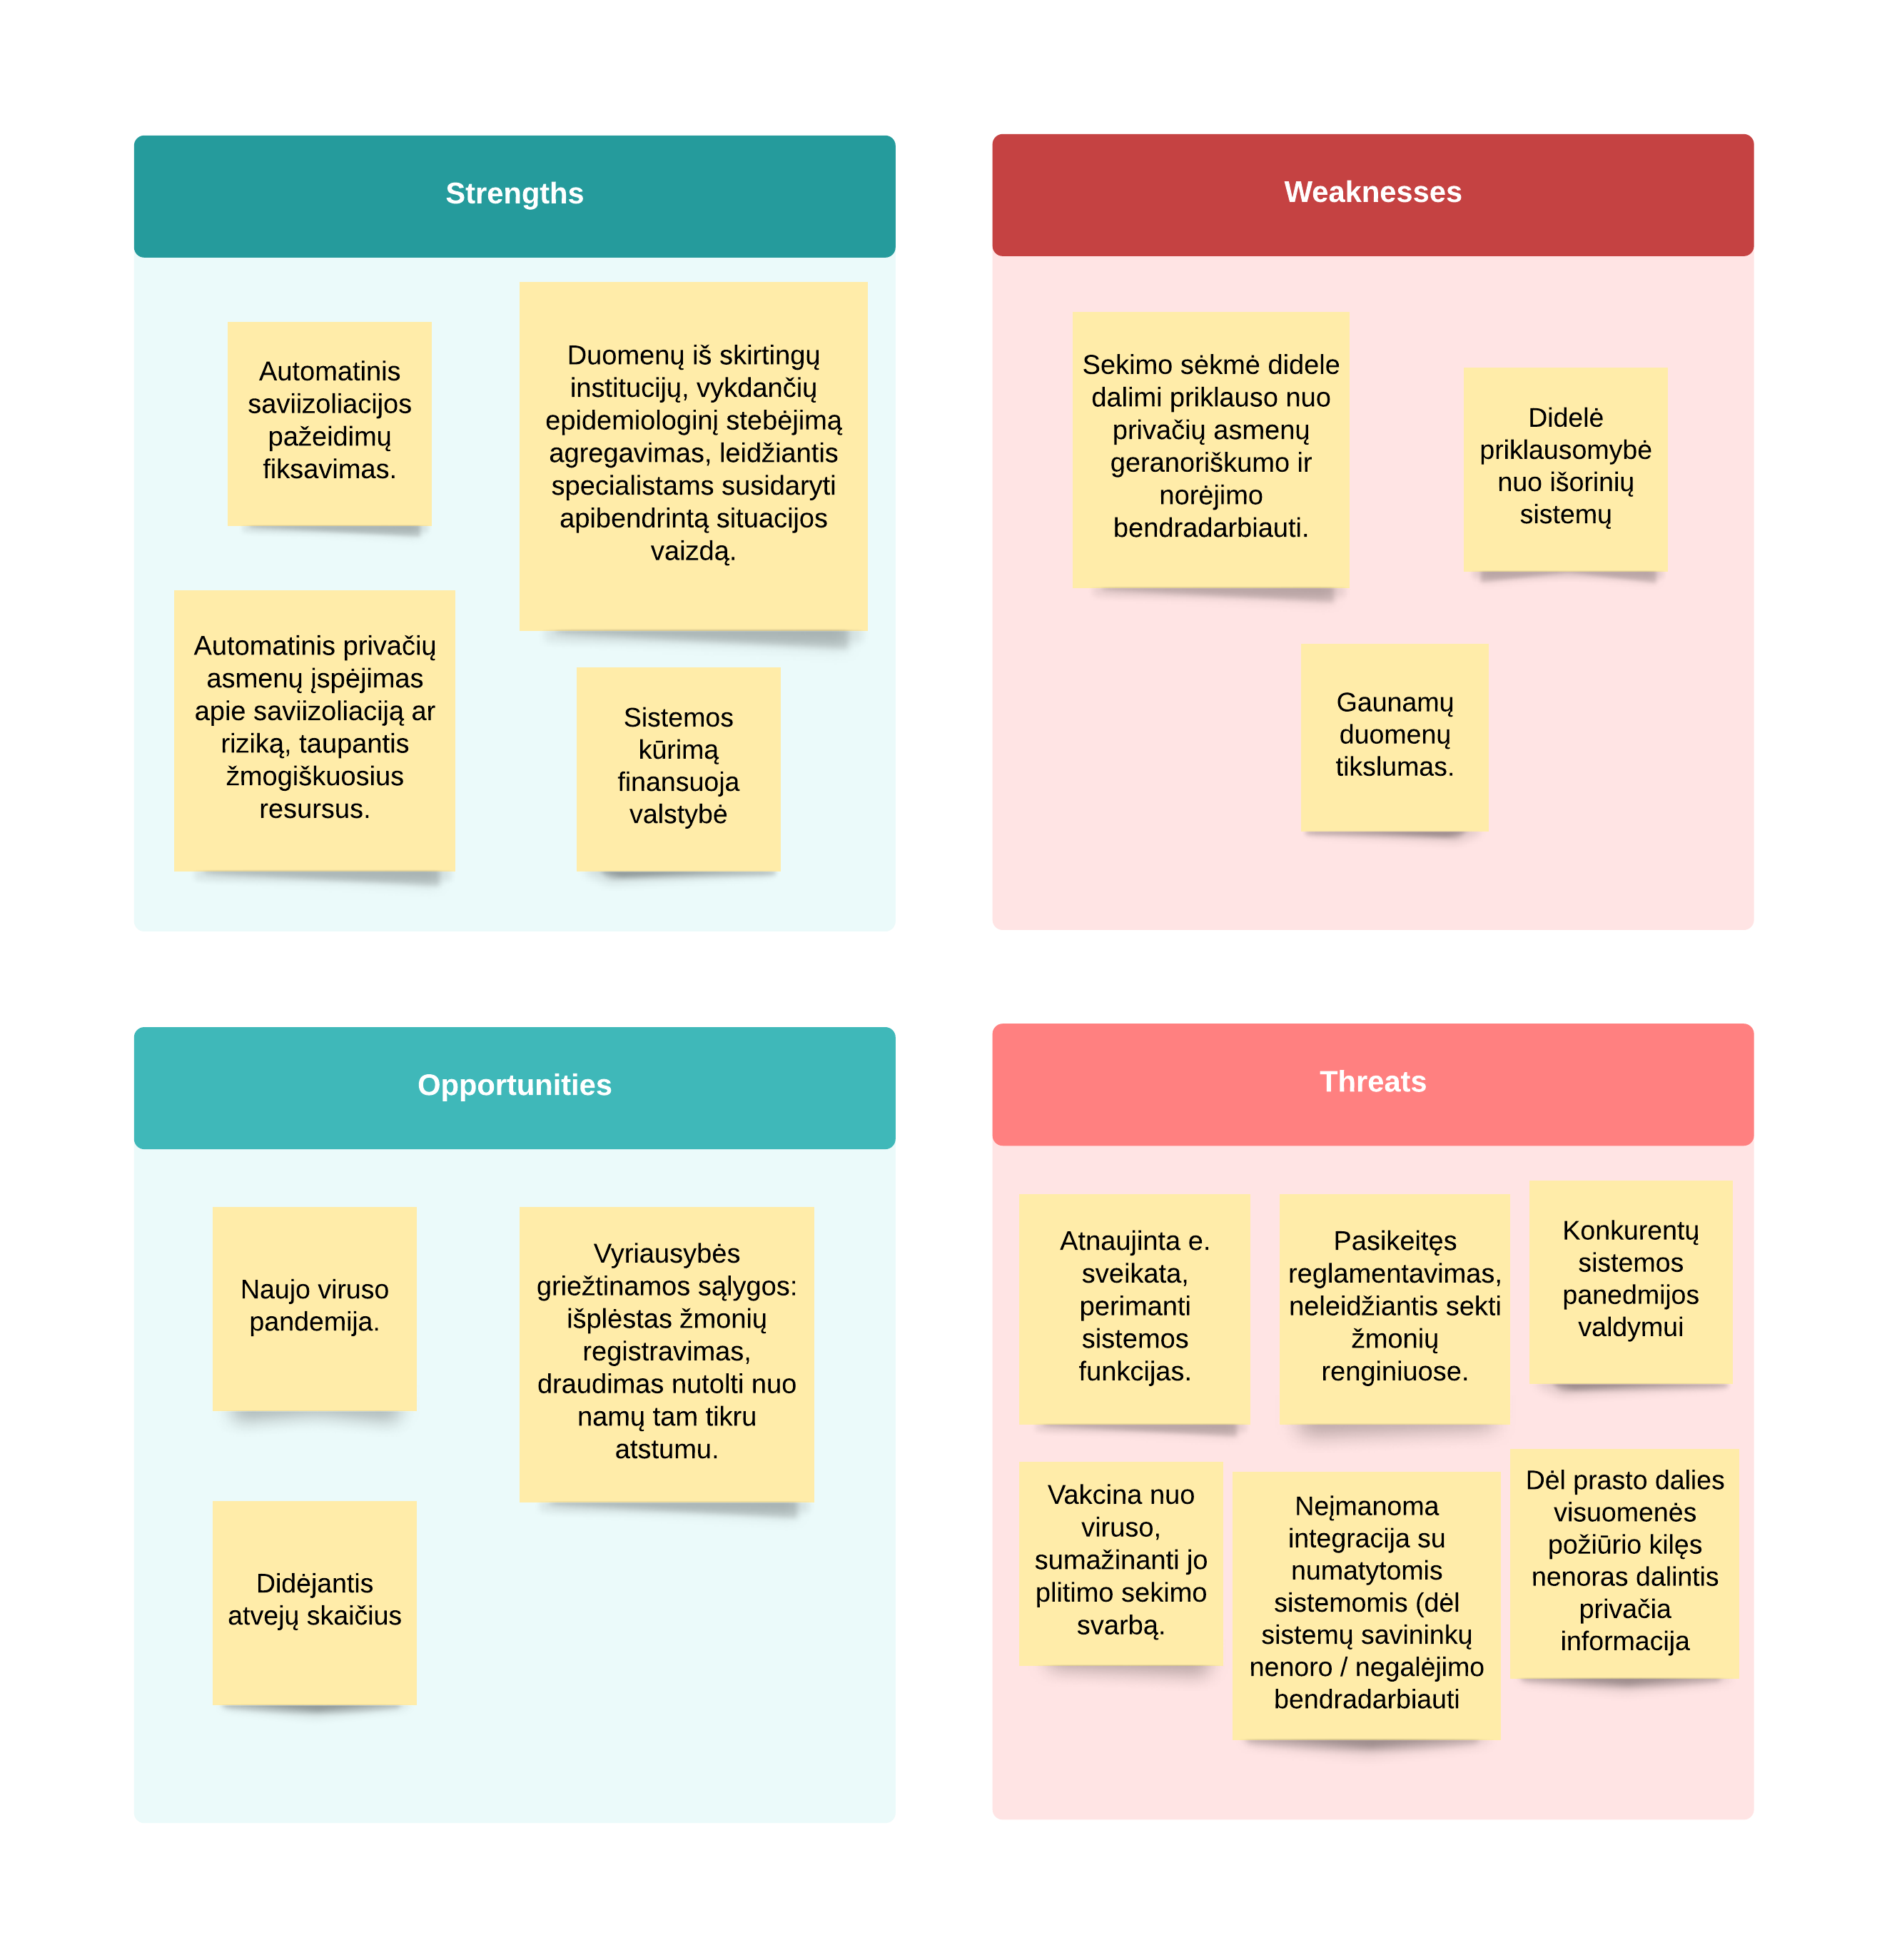
\includegraphics[scale=0.7]{img/SWOT.png}
    \caption{SWOT diagrama}
    \label{img:swot_diagram}
\end{figure}

\subsubsection{Siūloma verslo strategija}

\subsubsection{Tikslų medis}

\subsection{Kaip?}

\subsection{Kas?}

\subsection{Kieno?}

\subsection{Kur?}

\subsection{Kada?}

\end{document}

